\chapter{Evaluation}

\section{Reproduktion}
\label{reproduktion}

Der hier verwendete Simulationsaufbau erlaubt auf Wunsch eine deterministische sequentielle Ausführung. Dies erlaubt weiterführende Untersuchungen, die in Kapitel \ref{proptest} ausgeführt werden.

%\subsection{TLA+ Spec}
%Blabla bal
%bla
%TLA
%Mathematische spezifikation

\subsection{Simulations Aufbau}
Die Wahl des Paradigmas \ref{paradigma} fällt in dieser Arbeit auf das Ereignisorientiert Schema \ref{activity}. Dies mag erstaunen. Zunächst scheinen die Vorteile der Prozessorientierten Ansicht zu überwiegen. Im Falle eines verteilten Systems, wirkt die Modellierung durch Prozesse wie eine offensichtlich gute Wahl.
In Vorteile die sich ergeben, wenn man sich gegen diese Schema entscheidet, sind zweierlei.\\
Erstens, ist es dadurch leichter, nahe an einer Automaten-Spezifikation zu bleiben. Es bleibt die Sichtweise, das System als Zustand und einer Menge an möglichen Aktionen/Zustandsübergängen zu betrachten. Durch die Definition eines Standardverhaltens, nämlich zuerst alle fertigen Aufträge zu beenden, dann Aufträge zu starten, bis keine mehr startbar sind, und dann Menge an Zeiteinheiten vergehen zu lassen, erzielt man ein deterministisches Verhalten (solange die Scheduling Algorithmen deterministisch sind). Dieses reproduzierbare Verhalten ist gegenüber der Prozessorientierten Sicht ein Vorteil, da Fehler leichter gefunden und behoben werden können.\\
Zweitens leitet sich aus deterministischem Verhalten ein großer Vorteil für das Property Based Testing zum Erkenntnisgewinn in Kapitel \ref{proptest} ab.
Es werden ''flaky Tests'' verhindert, also Tests, die mit dem selben Systemzustand bei mehrfacher Ausführung sowohl fehlschlagen als auch gelingen. In diesen Fällen müssten sonst mehrere Tests durchgeführt werden.\\
Was das Shrinking in Kapitel \ref{proptest} angeht, könnte hier ein  Aktivitätsorientierter Ansatz Sinn ergeben, da immer kleinere Läufe erzeugt werden, sodass sich der Zusatzaufwand des Ereignisorientierte Paradigmas immer weniger lohnt. Jedoch ist dieser Overhead so gering, dass er im Vergleich zu den hohen Laufzeiteinbußen in der Ausführung von natürlichen Auftragslisten nicht ausschlaggebend ist.\\
Darüber hinaus lässt sich durch eine Alternative zum Standardverhaltens leicht untersuchen, wie sich das Verhalten des System ändert, wenn ein perfektes Betreiben des Clusters nicht möglich ist. Zum Beispiel kann überprüft werden, wie stark sich eine gröbere Zeitauflösung (etwa einmal alle 60 Sekunden) auf das Simulationsergebnis auswirkt. 


\subsection{Vergleich von Läufen}
\label{vergleich}
\subsubsection{Geschwindigkeit der Knoten}
Um abschätzen zu können, ob die vorgestellte Simulation erfolgreich reproduziert werden konnte, werden zuerst die Auswertungen von rein sequentiellen Auftragszusammenstellungen verglichen. Obwohl die Parameter zur Erstellung der Aufträge angegeben wurden, sowie die Tatsache, dass alle Knoten mit der selben Geschwindigkeit operieren, fehlt die Angabe über diese Geschwindigkeit. Experimentell lässt sich ermitteln, dass dieser Wert etwa $100$ beträgt.

\subsubsection{LPT, SPT}
\label{spt-lpt-time}
Bei Arndt et al. \cite[p.~4]{Arn99} wird zwischen der Bearbeitungszeit ("processing time") und der Laufzeit ("runtime") eines Auftrags unterschieden. Dabei bezeichnet Laufzeit den "Quotienten aus der Bearbeitungszeit $p_j$ und der kumulativen Geschwindigkeit der zugewiesenen Knoten". Das Ergebnis wird aufgerundet.\\
Bei der Simulation von SPT und LPT Läufen entstand folgendes Problem: Die Ergebnisse von Arndt et al. \cite{Arn99} ließen sich korrekt reproduzieren, solange alle Aufträge sequentiell waren. Sobald auch parallele Aufträge eingereiht wurden, entstanden geringe Abweichungen.\\
Es scheint, als würde der SPT Algorithmus in \cite{Arn99} nicht den Auftrag $j$ mit der geringsten Bearbeitungszeit $p_j$ auswählen, sondern denjenigen, der die geringste Zeit in Anspruch nimmt. Zum Beispiel würde $j_1$ mit $p_{j_1} = 10, \pi_{j_1} = 5$ gegenüber $j_2$ mit $p_{j_2} = 4, \pi_{j_1} = 1$ vorgezogen werden, da $j_1$ für $10/5 = 2$  Zeiteinheiten und $j_2$ für $4/1 = 4$ Zeiteinheiten ausgeführt wird.\\
Dies erfordert eine einfache Anpassung bzw. Interpretation des SPT Algorithmus. Es wird nach genannter Bearbeitungszeit geteilt durch den jeweiligen Grad an Parallelität sortiert. Diese Anpassung ergibt allerdings nur Sinn, solange alle Knoten mit der selben Geschwindigkeit arbeiten. Sobald Knoten unterschiedliche Geschwindigkeitseigenschaften besitzen, muss man die Bearbeitungszeit $j_p$ durch die Summe der Geschwindigkeiten der schnellsten freien Knoten teilen, um ein korrektes Ergebnis zu erhalten. Jedoch kann nun nicht bestimmt werden, wie lange ein Auftrag laufen wird, wenn nicht genügend Knoten zur Verfügung stehen. Zwar könnte man ähnlich dem Backfilling-Verfahren für jeden Auftrag vorhersehen, wann genügend Knoten bereitstehen werden, und dann die in der Zukunft freien Knoten zur Bestimmung der Laufzeit nutzen. Dies ist aber eine unverhältnismäßige Verkomplizierung eines eigentlich eleganten Algorithmus.\\
Dieses Problem wird auch in \cite{Arn99} beschrieben, und es wird ohne nähere Erläuterung angegeben, den ''statischen Bedarf'' der Aufträge zur Selektion zu verwenden. Aus diesen Gründen werden in dieser Arbeit LPT und SPT nach dem Quotienten aus Bearbeitungszeit und Parallelität ausgewählt. Dies erscheint wie eine sinnvolle Interpretation von ''statischem Bedarf''.
\subsubsection{Grafischer Abgleich Experimente 1,2 und 3}
Bevor das Simulationsmodell erweitert werden kann, sollte zuerst abgeglichen werden, ob das nachgebaute Modell näherungsweise ähnliche Läufe erzeugt. Dazu werden die in \cite{Arn99} beschriebenen Experimente nachgestellt, und die grafischen Auswertungen nebeneinander gestellt.
Da die Untersuchung des Random Schedulingalgorithmus im Verlaufe von \cite{Arn99} von Arndt aufgegeben wurde und mehr Läufe benötigt werden, um stabile Werte zu erzeugen, wird dieser hier nicht betrachtet.\\
Abbildungen eins bis drei \ref{figure1},\ref{figure2},\ref{figure3} lassen sich ohne Probleme, abgesehen von den nicht angegeben Geschwindigkeiten der Knoten, reproduzieren.
\begin{figure}
\centering
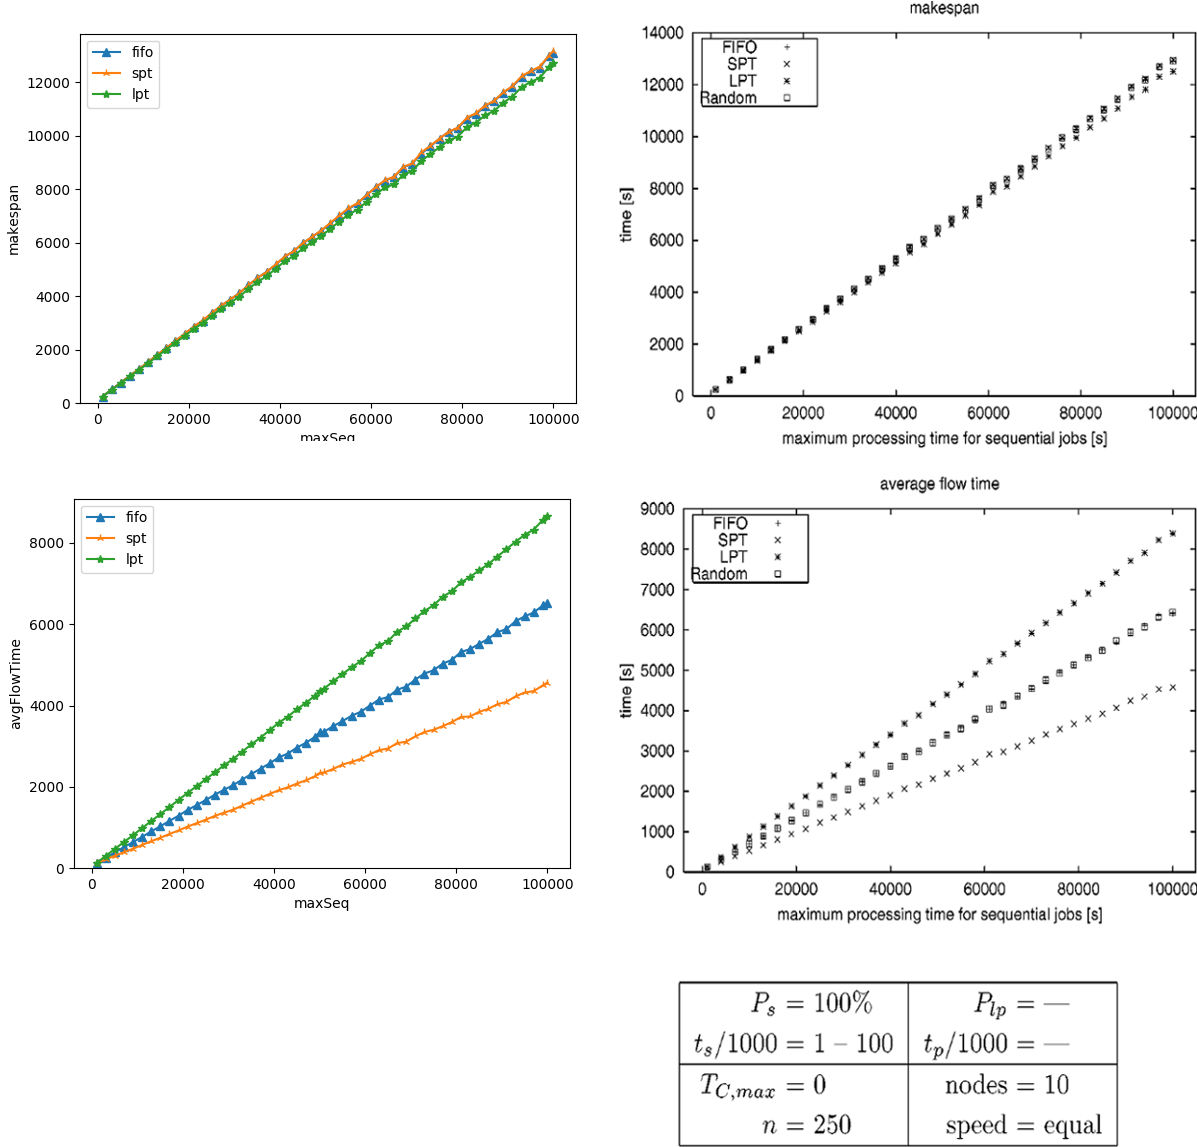
\includegraphics[width=\textwidth]{/home/hendrik/Programming/Python/BA/Docs/Hendrik/BA_Template/images/Figure_1.png}
\caption{Figure 1, Vergleich von sequentiellen Aufträgen nach Bearbeitungsspanne und längster Wartezeit}
\label{figure1}
\end{figure}
\begin{figure}
	\centering
	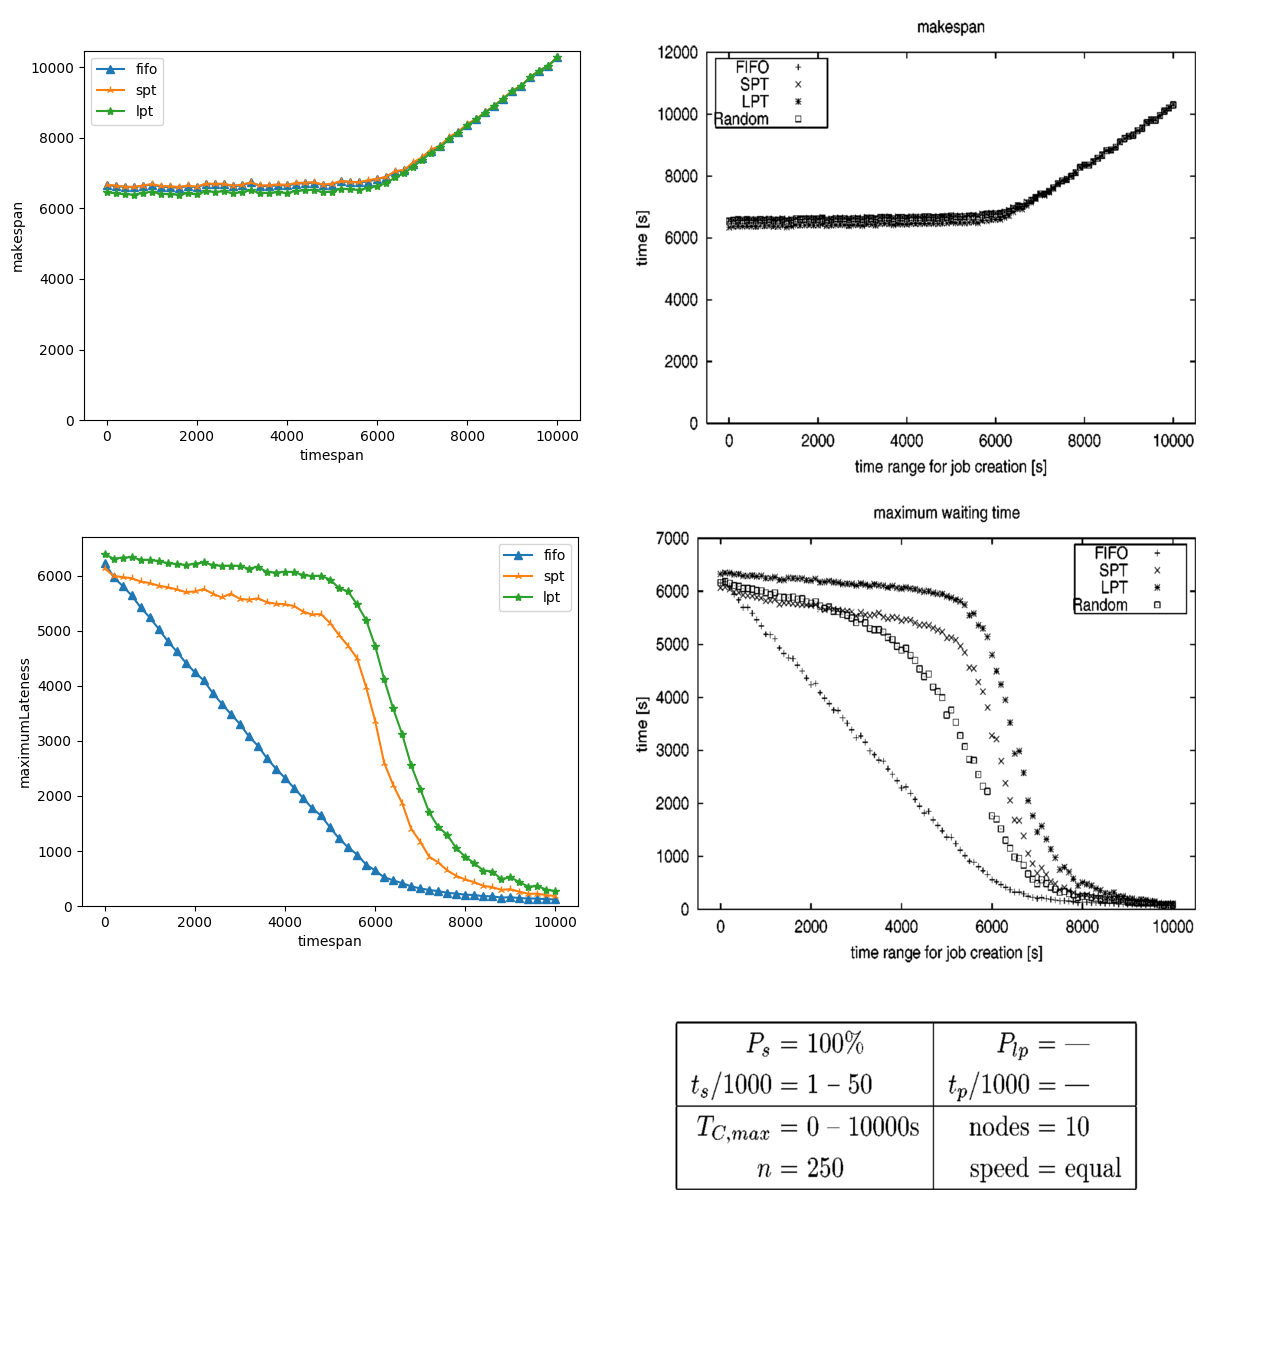
\includegraphics[width=\textwidth]{/home/hendrik/Programming/Python/BA/Docs/Hendrik/BA_Template/images/Figure_2.png}
	\caption{Figure 2, Vergleich von sequentiellen Aufträgen, nach Bearbeitungsspanne und längster Wartezeit, Erstellungszeit wird variiert}
	\label{figure2}
\end{figure}
\begin{figure}
	\centering
	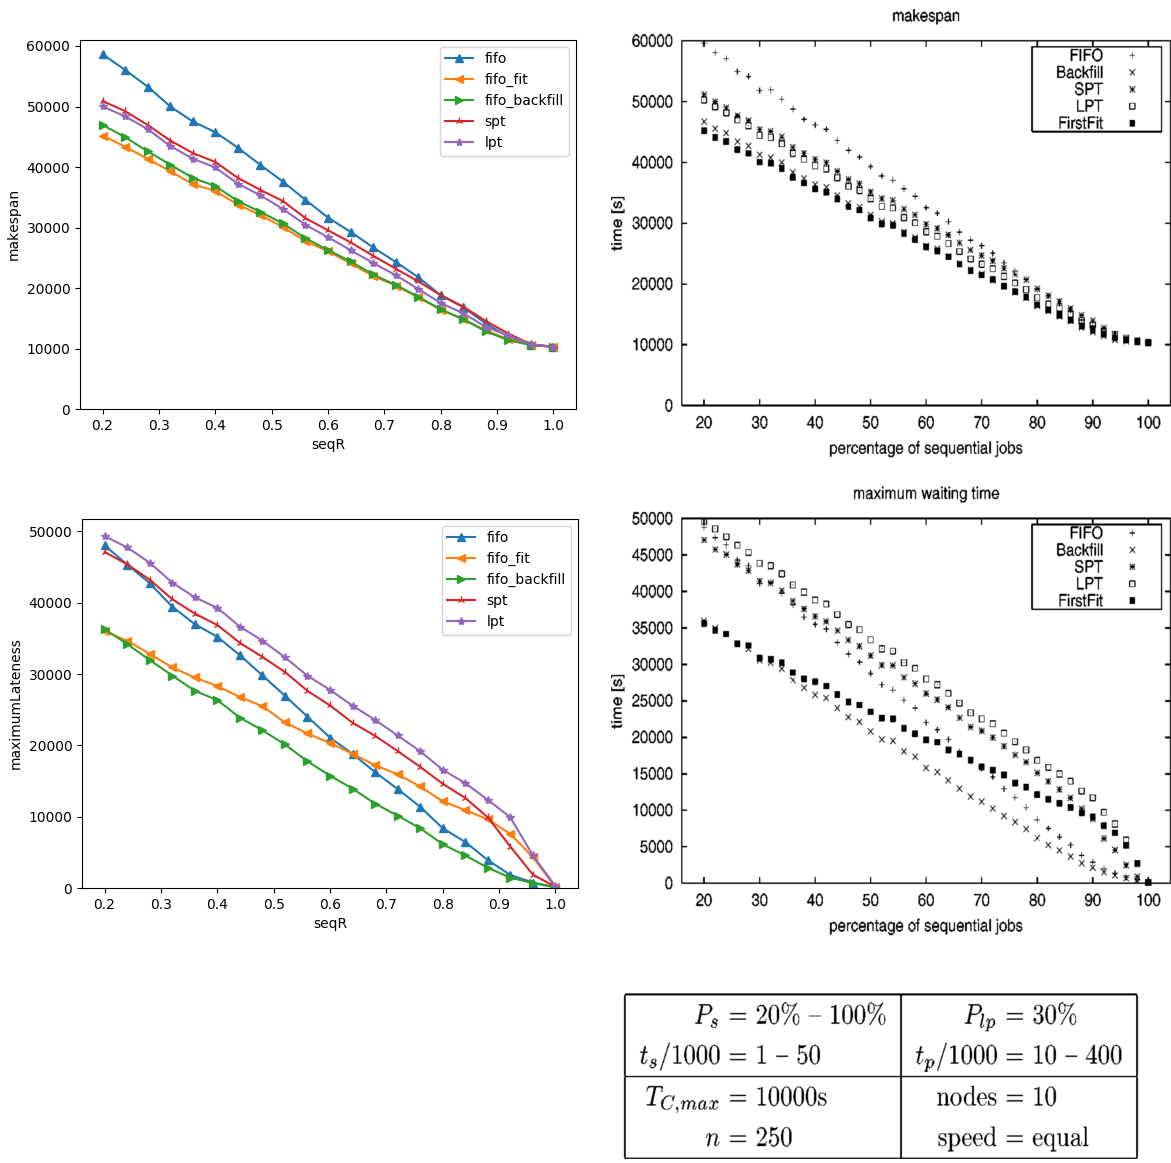
\includegraphics[width=\textwidth]{/home/hendrik/Programming/Python/BA/Docs/Hendrik/BA_Template/images/Figure_3.png}
	\caption{Figure 3, Vergleich von Sequentiellen Aufträgen nach längster Bearbeitungsspanne und längster Wartezeit, Anteil an sequentiellen Aufträgen wird zwischen 20\% und 100\% variiert}
	\label{figure3}
\end{figure}

\FloatBarrier

\subsubsection{Unterschiedlich schnelle Knoten ab Experiment 4}
Ab dem vierten Experiment offenbart sich folgendes Problem: Die Geschwindigkeiten der Knoten variieren. Sie entsprechen den Messungen von "22 Knoten des lokalen Netzwerks". Jedoch werden diese gemessen Geschwindigkeiten weder in der besprochenen, noch in früheren Veröffentlichungen dargelegt \cite{norepr1,norepr2}. Dies stellt eine hohe Hürde für die Reproduktion dar.\\

\begin{figure}
	\centering
	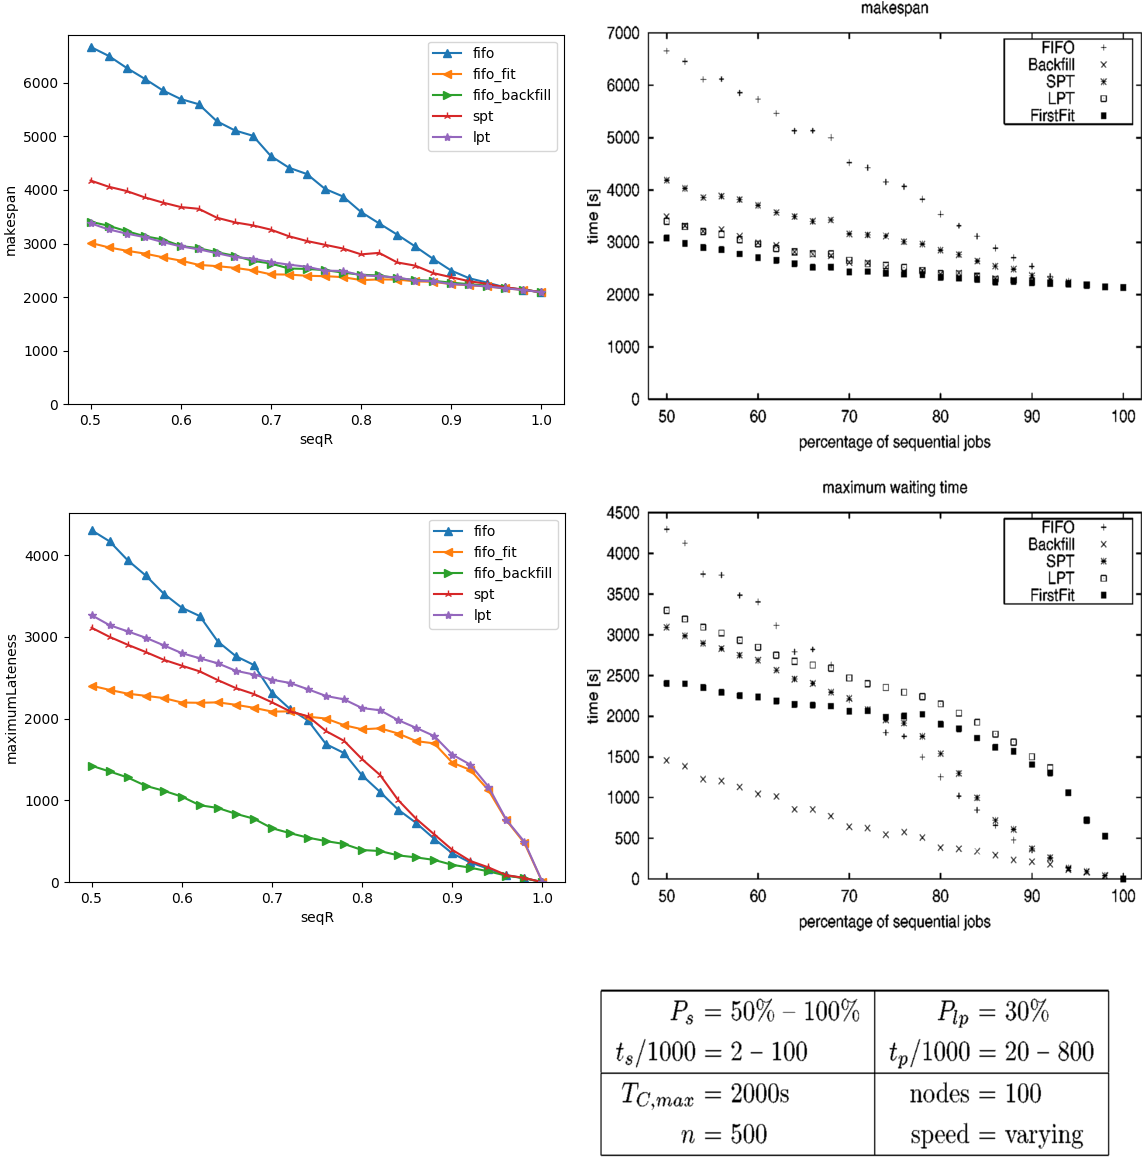
\includegraphics[width=\textwidth]{/home/hendrik/Programming/Python/BA/Docs/Hendrik/BA_Template/images/Figure_5}
	\caption{Unterschiedlich schnelle Knoten:\\
	75 Knoten mit Geschwindigkeit 275, 25 Knoten mit Geschwindigkeit 825}
	\label{figure5}
\end{figure}

Um die in Kapitel \ref{chap:higher-order} vorgeschlagenen Scheduler auch in den Experimenten 4 bis 9 bewerten zu können, wird eine ungefähre Verteilung der Geschwindigkeiten geschätzt.
Hierfür wird Abbildung 5 \ref{figure5} herangezogen. In diesem Experiment wird die Bearbeitungsspanne (makespan) angegeben. Dadurch lässt sich eine untere Schranke für die gesamte Rechenleistung des Clusters finden. Wenn durch FirstFit jeder Knoten zu jedem Zeitpunkt ausgelastet wäre, müsste die durchschnittliche Rechenleistung aller Knoten im beschriebenen Versuchsaufbau 384 betragen. Dies wird am Wert für einen Auftragsmix aus 50\% sequentiellen Aufträgen abgelesen. 100 Knoten unbekannter Geschwindigkeit benötigen etwa 3000 Sekunden um 500 Aufträge mit einer durchschnittlichen Bearbeitungszeit von 230500 Sekunden fertigzustellen. Um die durch die gierigen Algorithmen und die online eingehenden, also nicht von Anfang an bekannten Aufträge, entstehenden Effizienzeinbußen auszugleichen, wird die Geschwindigkeit der Knoten zusätzlich um 7,5\% erhöht. Der Anteil an ungenutzter Rechenzeit variiert je nach Experiment zwischen 2\% und über 50\%. Bei den 7,5\% handelt es sich also nicht um einen mathematisch begründeten Wert, sonder um einen empirisch ermittelten Wert, der plausible Ergebnisse liefert.
\begin{align*}
\frac{250*(51* 10^3 + 410*10^3)*s}{100x} &= 3000s \\
\frac{250*461}{300} &= x
\end{align*}
Die Frage nach der Art der verwendeten Verteilung lässt sich nicht klären. Deswegen wird hier die einfachste Verteilung gewählt: 2 Klassen von Knoten, mit unbekannten Geschwindigkeiten und Anzahlen. Der zweidimensionale Lösungsraum kann durch eine weitere Annahme auf einen eindimensionalen Raum reduziert: Die Menge der langsamen Knoten soll die selbe Gesamtleistung besitzen wie die Menge der schnellen Knoten.\\
Dies führt zu einer größeren Anzahl langsamer und einer geringeren Anzahl schnellerer Knoten. Diese Konstellationen sind sicherlich interessanter als ihre Umkehrungen. Gäbe es viele schnelle und wenige langsame Knoten, wären ähnliche Ergebnisse dadurch zu erreichen, die langsamen Knoten wegzulassen, wodurch sich die Situation nicht viel von den zuvor untersuchten unterscheiden würde.\\
Damit bleibt nur eine einzige Variable, der Anteil der langsamen Knoten im Cluster. Der Wert 0,75 erzeugt visuell vergleichbare Ergebnisse.

\FloatBarrier

\subsubsection{Experimente 4 bis 9}
Ab Experiment 4 kann keine Vergleichbarkeit der Modelle mehr sichergestellt werden. Trotzdem werden die Versuche nachgestellt, um die Algorithmen in \ref{chap:higher-order} gegen die fünf bekannten antreten zu lassen. Die Auswertung findet in \ref{weiter} statt.


\section{Weiterführende Untersuchungen}
\label{weiter}

\begin{figure}	
	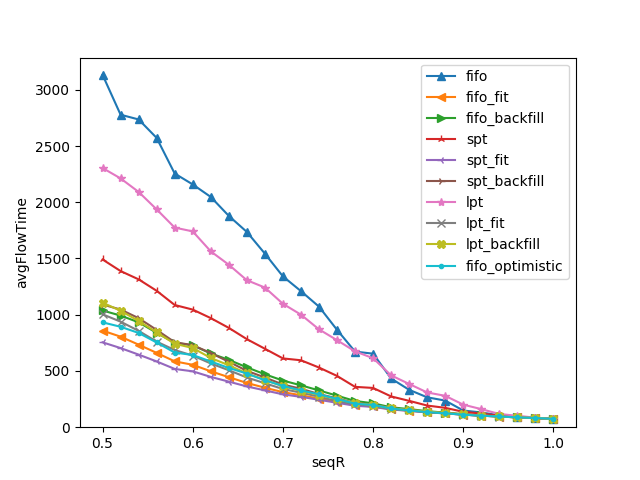
\includegraphics[width=\textwidth]{/home/hendrik/Programming/Python/BA/Docs/Hendrik/BA_Template/images/Figure_4_1}
	\caption{Varieren des Anteils von sequenziellen Aufträgen}
	\label{figure_4_1}
\end{figure}
\begin{figure}	
	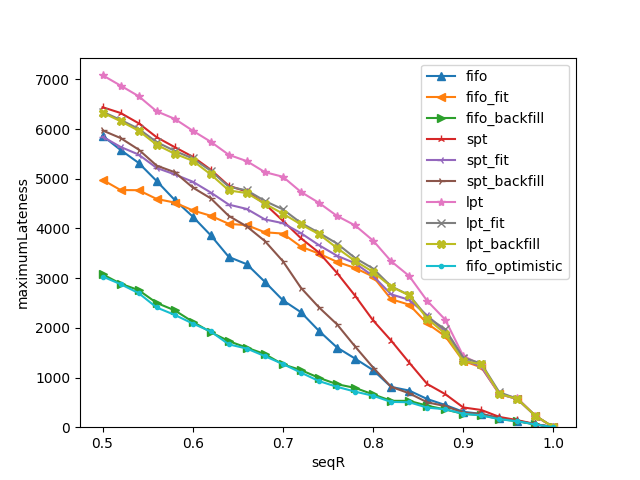
\includegraphics[width=\textwidth]{/home/hendrik/Programming/Python/BA/Docs/Hendrik/BA_Template/images/Figure_4_2}
	\caption{Varieren des Anteils von sequenziellen Aufträgen}
	\label{figure_4_2}
\end{figure}
\begin{figure}	
	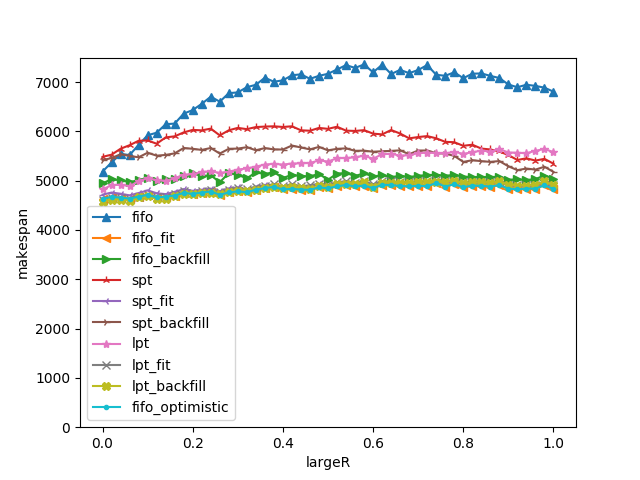
\includegraphics[width=\textwidth]{/home/hendrik/Programming/Python/BA/Docs/Hendrik/BA_Template/images/Figure_6_1}
	\caption{Varieren des Anteils von großen parallelen Aufträgen}
	\label{figure_6_1}
\end{figure}
\begin{figure}	
	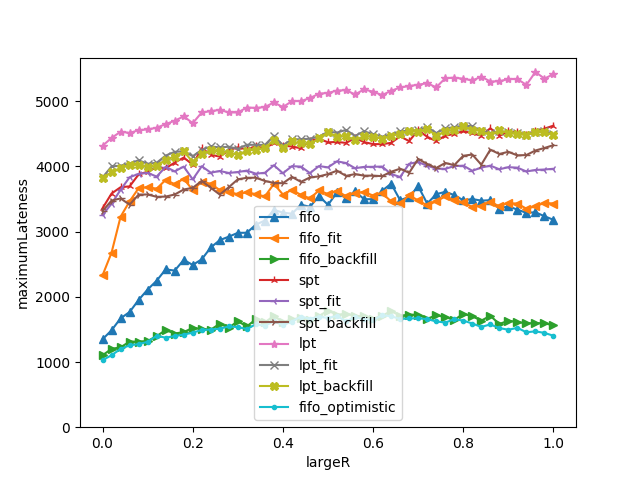
\includegraphics[width=\textwidth]{/home/hendrik/Programming/Python/BA/Docs/Hendrik/BA_Template/images/Figure_6_2}
	\caption{Varieren des Anteils von großen parallelen Aufträgen}
	\label{figure_6_2}
\end{figure}
\begin{figure}	
	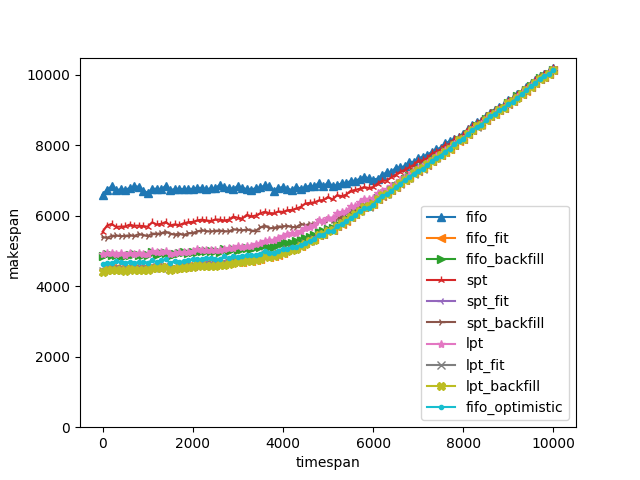
\includegraphics[width=\textwidth]{/home/hendrik/Programming/Python/BA/Docs/Hendrik/BA_Template/images/Figure_7_1}
	\caption{Varieren der Zeitspanne des Anmeldens von Aufträgen}
	\label{figure_7_1}
\end{figure}
\begin{figure}	
	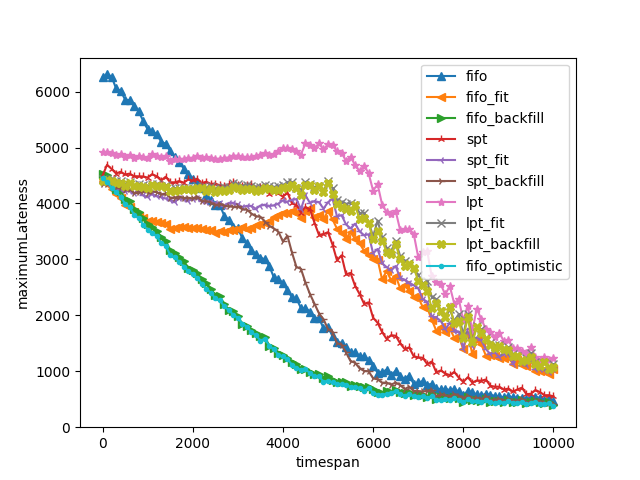
\includegraphics[width=\textwidth]{/home/hendrik/Programming/Python/BA/Docs/Hendrik/BA_Template/images/Figure_7_2}
	\caption{Varieren der Zeitspanne des Anmeldens von Aufträgen}
	\label{figure_7_2}
\end{figure}
\begin{figure}	
	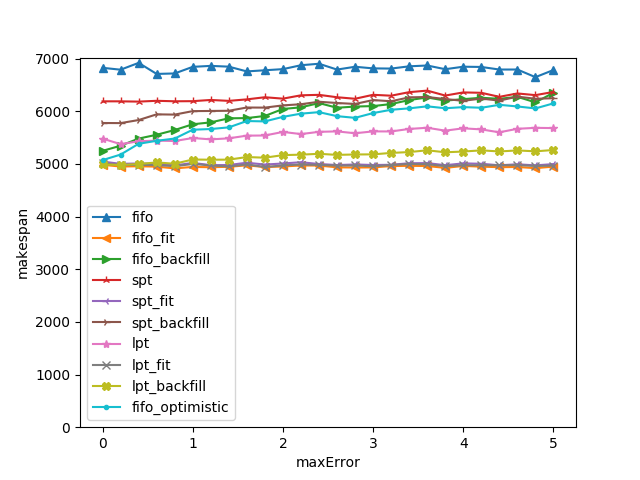
\includegraphics[width=\textwidth]{/home/hendrik/Programming/Python/BA/Docs/Hendrik/BA_Template/images/Figure_8_1}
	\caption{Varieren des erlaubten relativen Fehlers in der Angabe der Laufzeit}
	\label{figure_8_1}
\end{figure}
\begin{figure}	
	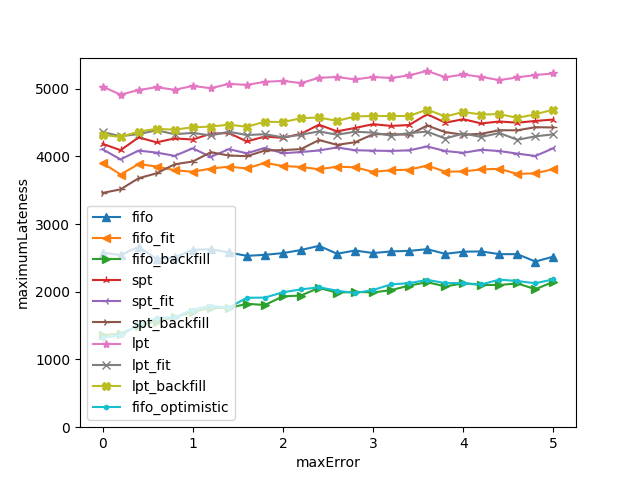
\includegraphics[width=\textwidth]{/home/hendrik/Programming/Python/BA/Docs/Hendrik/BA_Template/images/Figure_8_2}
	\caption{Varieren des erlaubten relativen Fehlers in der Angabe der Laufzeit}
	\label{figure_8_2}
\end{figure}


\FloatBarrier
\subsection{Backfilling und Fit als Funktionen höherer Ordnung}
\label{chap:higher-order}

Die in Kapitel 2 vorgestellten Funktionen FirstFit und Backfilling sind nur Abwandelungen der FiFo Funktion. Beide wählen den nächsten Auftrag abhängig vom Einreihungszeitpunkt $q_j$, jedoch unter Einschränkungen. ''FiFo-Fit'' wählt den ersten unter den startbaren Aufträgen aus, ''FiFo-BackFilling'' wählt den ersten Auftrag, oder einen, der den Bearbeitungsbeginn des ersten Auftrags nicht verzögert.\\ \mbox{''-Fit'' und ''-Backfilling''} fügen also einen relevanten Kontext hinzu. Es liegt nahe, diese Erweiterungen als Funktionen höherer Ordnung zu betrachten. Ihre Domäne besteht aus einer Scheduling Funktion, den wartenden Aufträgen und einen Kontext - Anzahl an verfügbaren Knoten oder die Abschlusszeitpunkte und die Parallelität der laufenden Aufträge -, und bilden diese partiell auf einen Auftrag ab. 
Da FirstFit-Backfilling von Arndt et al. als Sieger auserkoren wurde, LPT und SPT aber nicht im Backfilling Kontext untersucht wurden, wird im Folgenden untersucht, ob LPT oder SPT mit -FirstFit oder -Backfilling ähnlich gute Ergebnisse erzielen können.\\
Später \ref{optfill} wird eine Abwandlung des Backfillings vorgestellt, das optimistische Backfilling. Dieses wird in dieser Arbeit auch mit untersucht, allerdings hauptsächlich im FiFo Kontext.

\paragraph{SPT}
\label{spt-higher-order}
In Abbildung \ref{figure_4_1} wird die durchschnittliche Zeit eines Auftrags im System gemessen. Dabei schneidet SPT-Fit besser ab als alle anderen Algorithmen. Den zweiten Platz belegt FiFo-Fit. Für die durchschnittliche Systemzeit ist es wichtig, so schnell wie möglich Aufträge fertig zu stellen. Deshalb eigenen sich ''-Fit'' Funktionen, besonders in Kombination mit SPT. Erstaunlicherweise ist ''-Fit'' jedoch im Bezug zur Systemzeit nicht vollständig monoton. So gilt für die Messungen zwar SPT $<$ LPT $<$ FiFo, jedoch Fit$($FiFo$)$ $<$ Fit$($LPT$)$.\\
In Abbildung \ref{figure_7_2} erzielt SPT-Fit die selben Werte wie FiFo-Fit und LPT-Fit. In diesem Experiment wird die Bearbeitungsspanne in Abhängigkeit von einer relativen Fehlerrate in der Angabe von Bearbeitungszeiten ermittelt.\\


\paragraph{LPT}
In Abbildung \ref{figure_6_1} erzielen mehrere Algorithmen ähnlich  gute Ergebnisse. Darunter FiFo-Fit, SPT-Fit, LPT-Fit, LPT-Backfill und FiFo-Optimistic-Backfill. In diesem Experiment wird die Bearbeitungsspanne in Abhängigkeit des Anteils von großen parallelen Aufträgen gemessen. LPT-Fit ist hier deshalb eine gute Wahl, da LPT im Vergleich zu SPT und FiFo für eine geringere Spanne sorgt (vgl. auch \ref{figure3}). ''-Fit'' und ''-Backfill'' sorgt dafür, dass lange Phasen zum Anfang des Laufs, in denen einige Knoten nicht genutzt werden, während lange Aufträge abgearbeitet werden, gefüllt werden können.\\
Diese Beobachtung wiederholt sich in Abbildung \ref{figure_7_1}. Auch hier wird die Bearbeitungsspanne als Maß angelegt.\\


\paragraph{Optimistisches Backfilling}
Dieser Algorithmus wird in \ref{optfill} vorgestellt.\\
Beim Optimistischen Backfilling stellt sich vor allem die Frage, wie groß der Unterschied zum ''normalen'' Backfilling ist, und ob es sich die Bearbeitungsspanne verringert werden kann. Hierfür wurde nur FiFo in beiden Kontexten herangezogen.\\
In Abbildung \ref{figure_4_1} bietet das Optimistische Verfahren einen leichten, jedoch erkennbaren Vorteil. Hier wird die durchschnittliche Systemzeit von Aufträgen in Abhängigkeit des Anteils sequentieller Aufträge ermittelt. Es erscheint nachvollziehbar, dass, vorausgesetzt es gibt etwa gleich viele sequezielle und parallele Aufträge, eine Leistungssteigerung durch das Optimistische Verfahren erzielt werden kann. Das liegt daran, dass durch weniger Restriktionen mehr Lücken geschlossen werden können.\\
So auch in Abbildung \ref{figure_7_1}. Hier wird die gesamte Bearbeitungszeit in Abhängigkeit eines erlaubten Fehlers untersucht. Die selbe Argumentation erscheint plausibel. Wenn die Bearbeitungszeit eines Auftrags nicht korrekt angegeben wurde, werden weniger Aufträge gestartet um Lücken zu füllen. Das Optimistische Backfilling startet Aufträge, die wenige Knoten benötigen und nutzt so die Freiräume besser aus.\\
In allen anderen Versuchen ist kein nennenswerter Unterschied feststellbar. Es scheint, als wären die in Abschnitt \ref{optfill} genannten Konstellationen selten genug, als dass sie die nicht genutzten Chancen des ''normalen'' Backfilling überwiegen. Zumindest in den hier untersuchten Experimenten lässt sich die optimistische Variante als Ersatz empfehlen. In den meisten Fällen ist kein deutlicher Unterschied erkennbar, aber wenn, dann immer zu in Richtung geringerer Laufzeiten. Die detaillierte Untersuch der Auswirkung auf LPT und SPT übersteigen den Rahmen dieser Arbeit. 

\FloatBarrier

\paragraph{Backfilling und Fit von 2 Funktionen} Darüber hinaus ist es natürlich auch möglich, Backfilling und Fit in Abhängikeit von zwei Funktionen zu definieren. Das würde bedeutet, zuerst nach der ersten Funktion auszuwählen. Kann diese nicht gestartet werden, würde nach der zweiten Funktion aufgefüllt oder ein startbarer Auftrag gestartet. So könnten Schwächen einer Scheduling Funktion durch die Wahl einer anderen aufgewogen werden. Etwa könnten die längste Wartezeit des LPT-Backfill Algorithmus durch das Auffüllen nach FiFo verringert werden, die geringe Bearbeitungsspanne allerdings beibehalten werden. Alle Kombination zu vergleichen würde den Rahmen dieser Arbeit sprengen. Hier nun eine kurze erneute Betrachtung von Experiment \ref{figure_7_1}.\\
Es wird das bekannte FiFo-Fit, FiFo-Backfilling und LPT-Backfilling sowie das neue LTP-FiFo-Optimistisch in Abbildung \ref{figure_makespan} betrachtet. Dieses versucht einen Auftrag nach LPT auszuwählen. Kann dieser nicht gestartet werden, wird ein anderer Auftrag nach FiFo ausgewählt, der das bekannte optimistische Auffüll-Kriterium erfüllt.\\
Es fällt auf, dass LPT mit Backfilling tatsächlich eine geringere Bearbeitungsspanne erzielt, als FiFo-Backfilling. Darüber hinaus, konkurriert LPT-Backfilling mit FiFo-Backfilling bezüglich der durchschnittlichen Systemzeit. Der LPT Algorithmus, der nach FiFo auffüllt, stellt sogar eine kleine aber klare Verbesserung dar. Es lässt sich also sagen, dass sich LPT, insbesondere in Kombination mit FiFo, sehr gut eignet, um die Bearbeitungsspanne gering zu halten. Auch scheint das Auffüllen nach FiFo geringfügig fairer zu sein, als das normale Auffüllen mit LPT. Allerdings reicht dies nicht aus, um die Stärke des FiFo-Backfillings, nämlich die gute Ausnutzung der Ressourcen und die geringe längste Wartezeit, zu erreichen.
\begin{figure}	
	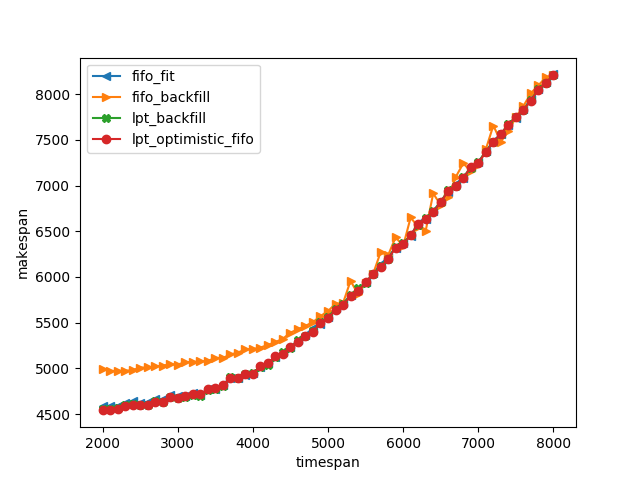
\includegraphics[width=\textwidth]{/home/hendrik/Programming/Python/BA/Docs/Hendrik/BA_Template/images/makespan.png}
	\caption{Variieren des Anmeldezeitraums}
	\label{figure_makespan}
\end{figure}
\begin{figure}	
	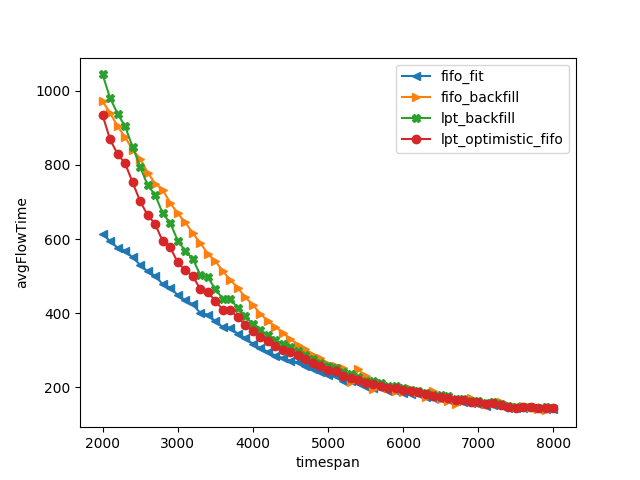
\includegraphics[width=\textwidth]{/home/hendrik/Programming/Python/BA/Docs/Hendrik/BA_Template/images/flowtime.png}
	\caption{Variieren des Anmeldezeitraums}
	\label{figure_flowtime}
\end{figure}
\begin{figure}	
	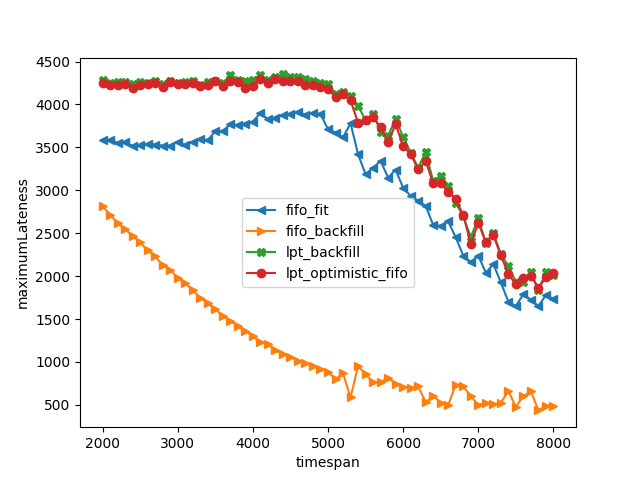
\includegraphics[width=\textwidth]{/home/hendrik/Programming/Python/BA/Docs/Hendrik/BA_Template/images/maxLate.png}
	\caption{Variieren des Anmeldezeitraums}
	\label{figure_maxLate}
\end{figure}


\FloatBarrier
\subsection{Property Based Testing zum Erkenntnisgewinn}
\label{proptest}
\paragraph{Testen statt Simullieren}
Während das Simulieren des Rechenclusters gute Auskunft darüber gibt, wie sich das System bei einer langen Reihe an Aufträgen verhält, kristallisiert sich dabei lediglich das durchschnittliche Verhalten heraus. Obwohl diese Analyse sinnvoll ist, um verschiedene Scheduling Funktionen asymptotisch miteinander zu vergleichen, wird durch das Mitteln von hunderten von Läufen nicht ersichtlich, in welchen Fällen eine normalerweise unterlegene Scheduling Funktion einer anderen überlegen ist.\\
Um eine Intuition für die Unterschiede zwischen Scheduling Funktionen entwickeln zu können ist es hilfreicher, die durch kleinstmögliche Listen an Aufgaben erzeugten Läufe zu vergleichen. Um diese minimalen Beispiele zu generieren, kann ein Property Based Testing Framework verwendet werden. Die zukunftsweisende Arbeit dieses Themas ist \emph{Quickcheck: a lightweight tool for random testing of haskell programs} \cite{hughes2000quickcheck}. Hier erfolgt nur eine kleine Zusammenfassung der Arbeit von John Hughes und Koen Claessen, der für dies Arbeit wichtigsten Aspekte aus. \\
Ein Test besteht aus einer zu testenden Funktion, eine Eigenschaft, die die Ausgabe der Funktion haben soll, und einem Generator, der Eingaben produziert. Sobald eine Eingabe gefunden wird, deren Ausgabe die geforderte Eigenschaft nicht erfüllt, wird die Eingabe automatisch geschrumpft. Dies führt zu einem leichter interpretierbaren Beispiel, da der ausgegebene Fall ''kein Rauschen'' enthält.
Eine Zahl wird geschrumpft, indem ihr Betrag reduziert wird, ein Tupel von Zahlen, indem eines der Elemente geschrumpft wird, und eine Liste, indem Elemente der Liste weggelassen oder geschrumpft werden.\\

Um ein minimales Beispiel zu finden, in dem Scheduling Funktion $S_1$ Ziel Funktion $T$ besser minimiert als Scheduler $S_2$, können wir die Eigenschaft $T(S_1(x)) >= T (S_2(1))$, mit einem Auftragsgenerator $X$: $(Anzahl Konten,[(\pi_j <= Anzahl Knoten,p_j,q_j)])$ überprüfen.
Ein vom Testframework gefundenes minimales Gegenbeispiel, zeigt uns einen speziellen Fall, in dem $S_1$ ein besseres Ergebnis erzielt als $S_2$ (\cite{TestOpt}).
Für die meisten Scheduling Funktionen ist das Minimalbeispiel eines mit 3 Aufträgen, und einer kleinen Anzahl an Knoten.

Hier nun einige Beispiele:\\

\paragraph{Optimistisches Backfilling}
\label{optfill}
Das vorgestellte ''-Backfilling'' Verfahren wirkt auf den ersten Blick zurückhaltend. Das angegebene Ziel, die zum ''-Fit'' verglichene Wartezeit gering zuhalten, wird erfüllt, indem große Aufträge nicht benachteiligt werden. Kleine werden nur vorgezogen, wenn sich dadurch die Wartezeit des besten, aber nicht startbaren Kandidaten, nicht verzögert. Dies wird erreicht, indem ein Auftrag $P'$ nur starten darf, wenn er abgeschlossen wird, bevor der beste Kandidat $P$ startet.\\
Warum aber darf ein Auftrag $P'$, der wenige Knoten benötigt, nicht starten, vorausgesetzt, er nimmt nur so wenige Knoten in Anspruch, dass $P$ wie geplant starten kann ($P$ benötigt noch $n$ Knoten zum starten, sobald er starten wird, sind aber $n+k, k>0$ Knoten frei, und $\pi_{P'} <= k$) vgl. 
Von Arndt et al. wird bezüglich dieser Idee auf \cite{optVsCons} verwiesen.\\
Es ist intuitiv, dass es einen Haken gibt. Es ist aber nicht einfach, aus dem Stand ein Beispiel zu konstruieren, in dem sich das optimistische -Backfilling negativ auf die Wartezeit auswirkt. Allerdings kann dank Property Based Testing eines in wenigen Sekunden generiert werden.

\begin{figure}
\centering
\begin{verbatim}
Is fifo\_optimistic allways better than
 fifo\_backfill by maximumLateness?
No! counterexample:
queueintT, processingT, realProcessingT, degreeOfParallelism
id: 0, qT: 1, pT: 3, rPT: 3, doP: 1
id: 1, qT: 0, pT: 3, rPT: 3, doP: 2
id: 2, qT: 0, pT: 1, rPT: 1, doP: 2
id: 3, qT: 0, pT: 1, rPT: 1, doP: 3

maximumLateness of fifo\_optimistic: 4
[0]:112|-3
[1]:112|-3
[2]:-00|03

maximumLateness of fifo\_backfill: 3
[0]:112|3--|-
[1]:11-|300|0
[2]:--2|3--|-
\end{verbatim}
\caption{Vergleich vom Normalem und Optimistischem Backfilling}
\label{onlateness}
\end{figure}

\FloatBarrier

Hier ist der optimistische Algorithmus zu voreilig. Auftrag 0 wird gestartet, obwohl er (als einziger) nicht seit Beginn angemeldet ist. Dadurch wird Auftrag 3 nach hinten geschoben und die maximale Wartezeit für 3 steigt. Trotzdem ist die Auslastung des optimistischen Algorithmus deutlich besser. Doch existiert auch einen Fall, in dem sowohl die maximale Verspätung, als auch die gesamt Bearbeitungszeit schlechter sind?\\


\begin{figure}
\centering
\begin{verbatim}
Is fifo_optimistic allways better than <function System.fifo_backfill at 0x7f42574fd7b8> by <function maximumLateness at 0x7f42408ff400> ?
No! counterexample:

queueintT, processingT, realProcessingT, degreeOfParallelism
id: 0, qT: 1, pT: 1, rPT: 1, doP: 4
id: 1, qT: 1, pT: 3, rPT: 3, doP: 1
id: 2, qT: 1, pT: 3, rPT: 3, doP: 1
id: 3, qT: 0, pT: 4, rPT: 4, doP: 3
id: 4, qT: 0, pT: 1, rPT: 1, doP: 2

maximumLateness offifo_optimistic: 4
makespan of fifo_optimistic: 8
[0]:334|-0-|--
[1]:334|-0-|--
[2]:33-|-02|22
[3]:-11|10-|--

maximumLateness offifo_backfill: 3
makespan of fifo_backfill: 7
[0]:334|0--|-
[1]:33-|011|1
[2]:33-|022|2
[3]:--4|0--|-
\end{verbatim}
\caption{Vergleich vom Normalem und Optimistischem Backfilling in Spanne und Verspätung}
\label{onlatenessmakespan}
\end{figure}

Auch hier kann ein durch Property Based Testing ein Fall konstruiert werden. Allerdings besteht hier das kleinste gefundene Beispiel bereits aus 5 Aufträgen. Es ist also zu erwarten, dass solche Konstellationen selten genug sind. Eine genauere Untersuchung dazu im Abschnitt \ref{chap:higher-order}.
\FloatBarrier

Wie in der Grafik \ref{onlateness} nach einem Schritt erkennbar, benachteiligt ein solcher optimistisch gestarteter langer, kleiner Auftrag nicht den besten Kandidaten (Auftrag 4), allerdings den zweitbesten Kandidaten (Auftrag 0). Ob dies ein seltener Fall ist, oder ob sich Optimismus im Mittel auszahlt, kann wiederum durch eine Statistische Auswertung untersucht werden.\\

Außerdem ist es interessant zu beobachten, welche Informationen implizit aus diesem Gegenbeispiel gezogen werden können. Zum Beispiel, dass im ersten Lauf \ref{onlateness} nur ein einziger online Auftrag (d.h. nicht schon zum Zeitpunkt 0 bekannt) nötig ist, aber um das optimistische Verfahren in beiden Metriken zu schlagen, werden 3 online Aufträge sowie ein zusätzlicher Auftrag benötigt. Es fällt auch auf, dass in diesem Beispiel FiFo-Backfill nie vom Backfilling Gebrauch macht. Es verhält sich immer wie das blanke FiFo Verfahren. Warum also nicht einen Auftragsmix finden, in dem das normale Backfilling sowohl FiFo als auch das optimistische Backfilling trumpft, und zwar sowohl was die Bearbeitungsspanne als auch die längste Wartezeit angeht? Auch hier soll der Leser aufgefordert sein, selber nach einem Beispiel zu suchen.\\

\begin{figure}
	\centering
	\begin{verbatim}
id: 0, qT: 0, pT: 1, rPT: 1, doP: 2
id: 1, qT: 0, pT: 1, rPT: 1, doP: 3
id: 2, qT: 0, pT: 2, rPT: 2, doP: 1
id: 3, qT: 0, pT: 1, rPT: 1, doP: 3
id: 4, qT: 0, pT: 1, rPT: 1, doP: 2

maximumLateness of fifo_optimistic : 3
makespan of fifo_optimistic : 4
[0]:013|4
[1]:013|4
[2]:223|-
[3]:-1-|-

maximumLateness of fifo_backfill : 2
makespan of fifo_backfill : 3
[0]:013
[1]:013
[2]:413
[3]:422

maximumLateness of fifo : 3
makespan of fifo : 4
[0]:013|4
[1]:013|4
[2]:-13|-
[3]:-22|-
\end{verbatim}
\caption{Backfill besser als Optimistic und Fifo, bez. Bearbeitunsspanne und längster Wartezeit}
\label{everything}
\end{figure}

Des weiteren fällt auf, dass das Shrinking Verfahren herausgefunden hat, dass zur Berechnung der Laufzeiten von parallelen Aufträgen aufgerundet wird (s. \ref{spt-lpt-time}). Da dies der Lesbarkeit der Tests zuwider läuft, kann die Bearbeitungszeit jedes Auftrags einfach auf das nächste Vielfache der Parallelität gesetzt werden.
Zusätzlich wird oft die Gleichstände-auflösenden Ids zurückgegriffen. Es kann explizit gefordert werden, dass alle Einreihungszeitpunkte der Aufträge verschieden sind. Allerdings verlangsamt dies die Suche nach einem Gegenbeispiel, und das kleinste gefundene Gegenbeispiel hat eine Bearbeitungsspanne von 13 Zeiteinheiten oder mehr.\\
\FloatBarrier

\subsection{Vergleich von Simulation und PBT}
\label{prop-sim}
Die Simulation vergleicht Scheduling Algorithmen anhand ihrer Leistung beim Bearbeiten von -  konstruierten - Auftragszusammenstellungen. Das PBT findet zu Scheduling Algorithmen einen dazu passenden Auftrags- und Knotenmix, in dem sich die Leistungen unterscheiden. Rückschlüsse können basierend auf der Komplexität dieser Szenarien gezogen werden. Die Vermutung, dass komplizierte, oder gestellt Konstellationen im Normalbetrieb selten sind, und dass ein Algorithmus, der nur in solchen Situationen zu schlagen ist, sich auch im Normalbetrieb bewährt, ist noch zu überprüfen.\\

Vorab ist zu wählen, nach welcher Zielfunktion bemessen werden soll. Da auch \cite{Arn99} sich vor allem auf die Bearbeitungsspanne konzentrieren, wollen wir das hier auch tun. Außerdem ist auch zu klären, was die kleinste Situation ist, in dem zwei verschieden Scheduler zwei verschiedene Ergebnisse liefern. Offensichtlich müssen dafür mindestens zwei Knoten beteiligt sein, und mehr als 2 Aufträge vorhanden sein. Zunächst wird diese Überlegung überprüft. Dafür wird ein neuer Scheduler ’’FId’’ geschaffen, der immer den Auftrag mit der niedrigsten Id auswählt. Dann wird nach einem Test gesucht, in dem sich ein FId System anders verhält, wenn die Ids in der Auftragsliste vor Start der Simulation permutiert werden. Diese Vermutung lässt sich schnell durch einen Versuch bestätigen (s. \ref{minX}).\\
\begin{figure}
\centering
\begin{verbatim}
makespan : 2
id: 0, qT: 0, pT: 1, rPT: 1, doP: 2
id: 1, qT: 0, pT: 1, rPT: 1, doP: 1
id: 2, qT: 0, pT: 1, rPT: 1, doP: 1
[0]:01
[1]:02

makespan : 3
id: 0, qT: 0, pT: 1, rPT: 1, doP: 1
id: 1, qT: 0, pT: 1, rPT: 1, doP: 2
id: 2, qT: 0, pT: 1, rPT: 1, doP: 1
[0]:012
[1]:-1-
\end{verbatim}
\caption{minimales Beispiel, in dem sich die Wahl der Scheduling Funktion auswirkt}
\label{minX}
\end{figure}

Nun können bisher vorgestellten Scheduler miteinander verglichen werden. Die "Gestelltheit" des kleinsten Beispiels setzt sich dabei aus der Anzahl an Aufträgen, Knoten, und online Aufträgen zusammen. Hier sei noch angemerkt, dass dies, ebenso wie das Simulieren, keine exakten Ergebnisse liefert. Es ist immer möglich, dass es einen noch einfacheren Fall gibt, den das Shrinking Verfahren nicht gefunden hat. Es werden für jede Paarung 100.000 Beispiele ausprobiert. Ebenso gibt es mehrere kleinste Beispiele. Zum Beispiel kann FiFo LPT mit 
3-2-1 oder 4-2-0 schlagen. Das Shrinking Verfahren betrachtet dabei ersteres Ergebnis als "kleiner". Hierfür kann ''gezieltes PBT'' (\cite{testTarget}) verwendet werden. Hierbei wird ein Wert angegeben, den das Test Framework minimiert, zum Beispiel die Differenz zwischen den zwei Bearbeitungsspannen. Dadurch verringert sich zwar die Zeit, die gebraucht wird, um ein Gegenbeispiel zu finden, allerdings variiert dadurch die Größe der Beispiele stärker. Aus diesem Grund wird darauf hier verzichtet.\\


\begin{table}[]
	\resizebox{\textwidth}{!}{\begin{tabular}{lllllllllll}
		\hline
		J+k+o      & fifo  & spt   & lpt   & Fifo-fit & Fifo-back & Fifo-optim & Spt-fit & Spt-back & Lpt-fit & Lpt-back \\ \hline
		fifo       & +     & 3+2+0 & 3+2+1 & 6+2+2    & X         & 8+3+4      & 3+4+0   & 3+2+0    & 3+2+1   & 3+9+1    \\
		spt        & 3+2+1 & +     & 3+2+1 & 4+2+1    & 4+2+1     & 4+2+1      & 6+8+0   & 6+10+5   & 3+3+1   & 4+5+3    \\
		lpt        & 3+2+0 & 3+2+0 & +     & 4+4+2    & 3+2+0     & 3+2+2      & 3+2+0   & 3+2+0    & 4+2+2   & 7+5+2    \\
		Fifo-fit   & 3+2+2 & 3+2+2 & 3+2+0 & +        & 5+4+2     & 3+2+1      & 3+2+0   & 3+2+0    & 3+2+1   & 4+3+0    \\
		Fifo-back  & 5+2+0 & 3+2+2 & 3+2+0 & 5+6+4    & +         & 7+6+2      & 3+3+0   & 3+2+2    & 3+2+1   & 3+2+1    \\
		Fifo-optim & 3+3+1 & 3+2+0 & 3+2+0 & 4+2+1    & 3+4+0     & +          & 3+4+0   & 3+2+2    & 3+2+1   & 3+2+1    \\
		Spt-fit    & 3+2+2 & 3+2+2 & 3+2+0 & 3+2+1    & 3+2+2     & 3+2+0      & +       & 3+3+0    & 3+2+1   & 5+5+4    \\
		Spt-back   & 3+2+0 & 5+2+2 & 3+2+1 & 3+2+1    & 3+2+1     & 3+2+1      & 5+4+2   & +        & 3+2+1   & 3+2+1    \\
		Lpt-fit    & 3+2+2 & 3+2+1 & 3+2+0 & 3+2+0    & 3+2+1     & 3+2+0      & 3+2+0   & 3+2+0    & +       & 4+4+3    \\
		Lpt-back   & 3+2+1 & 3+2+2 & 3+3+0 & 3+2+0    & 3+4+1     & 4+2+1      & 3+2+0   & 3+2+0    & 5+4+2   & +        \\ \hline
	\end{tabular}}
	\caption{Größe des kleinsten gefundenen Falls, in dem Spalte eine kleinere Spanne hat als Zeile}
	\label{tabAbsFit}
\end{table}

\begin{table}[]
	\resizebox{\textwidth}{!}{\begin{tabular}{lllllllllllll}
		\cline{1-13}
		& V/G & fifo & spt & lpt & Fifo-fit & Fifo-back & Fifo-optim & Spt-fit & Spt-back & Lpt-fit & Lpt-back &  \\ \cline{1-13}
		0.756 & fifo & 0 & 5 & 6 & 10 & nn & 15 & 7 & 5 & 6 & 13 & 8.375 \\
		0.667 & spt & 6 & 0 & 6 & 7 & 7 & 7 & 14 & 21 & 7 & 12 & 9.667 \\
		0.766 & lpt & 5 & 5 & 0 & 10 & 5 & 7 & 5 & 5 & 8 & 14 & 7.111 \\
		1.203 & Fifo-fit & 7 & 7 & 5 & 0 & 11 & 6 & 5 & 5 & 6 & 7 & 6.556 \\
		0.867 & Fifo-back & 7 & 7 & 5 & 15 & 0 & 15 & 6 & 7 & 6 & 6 & 8.222 \\
		1.281 & Fifo-optim & 7 & 5 & 5 & 7 & 7 & 0 & 7 & 7 & 6 & 6 & 6.333 \\
		1.032 & Spt-fit & 7 & 7 & 5 & 6 & 7 & 5 & 0 & 6 & 6 & 14 & 7 \\
		1.082 & Spt-back & 5 & 9 & 6 & 6 & 6 & 6 & 11 & 0 & 6 & 6 & 6.778 \\
		1.127 & Lpt-fit & 7 & 6 & 5 & 5 & 6 & 5 & 5 & 5 & 0 & 11 & 6.111 \\
		1.483 & Lpt-back & 6 & 7 & 6 & 5 & 8 & 7 & 5 & 5 & 11 & 0 & 6.667 \\ \cline{1-13}
		&  & 6.333 & 6.444 & 5.444 & 7.889 & 7.125 & 8.111 & 7.222 & 7.333 & 6.889 & 9.889 & 
	\end{tabular}}
	\caption{Durchsnittliche Größe jeder Zeile und Spalte; links das Verhältnis aus durchschn. Gewinn und Verlierer Größe}
	\label{tabRelFit}
\end{table}

Hierbei ist zu beachten, dass FiFo nie seine Backfill-Variante besiegen kann. Dies liegt daran, dass das Auswahlkriterium von FiFo die Einreihungszeit ist. Per Definition kann also kein online eingereihter Auftrag erscheinen, der dieses Kriterium besser erfüllt, als die bereits bekannten Aufträge. Für SPT und LPT gilt dies nicht.\\
Aus diesem Grund wird hier der Durchschnitt der nicht-null Werte verrechnet. Dies benachteiligt FiFo-Backfill und bevorteilt FiFo. Alternativ wäre eine Betrachtung ohne den FiFo Algorithmus möglich.\\
Als zweites fällt die Wahl eines Versuchsaufbau an, mit dem der Property Based Testing score (pbt-score) verglichen werden soll. Das PBT Werkzeug darf folgende Freiheiten ausnutzen: Anzahl an Knoten, Dauer, Einreihungszeitpunkt und Parallelität der Aufträge. Fest steht die Geschwindigkeit der Knoten, in diesem Fall der Lesbarkeit wegen 1. Ebenso wurden alle Bearbeitungszeiten korrekt angegeben. Aus diesem Grund wird Experiment 3 gewählt \ref{figure3}. In diesem haben alle Knoten die selbe Geschwindigkeit, der Anteil an sequentiellen Aufträgen wird variiert und 30\% der parallelen Aufträge nehmen mindestens die Hälfte der Knoten in Anspruch. Das Experiment wird wiederholt, diesmal mit zusätzlichen Scheduling Algorithmen. Es wird ein quantitativer Wert zur Berechnung der Korrelation benötigt. Hierfür wird das Integral der verschiedenen Grafen berechnet, anstatt die Bearbeitungsspanne an einem willkürlich gewählten Punkt zu messen.
Die Ergebnisse befinden sich in Tabelle \ref{rank}. Der \emph{Rangkorrelationskoeefizients nach Spearman} von \emph{-1}  legt eine starke negative Korrelation nahe. \\

\begin{table}[]
		\resizebox{\textwidth}{!}{\begin{tabular}{lllll}
		\hline
		algorithm                         & area under curve & pbt score         & a.u.c. Rank & pbt Rank \\ \hline
		fifo      & 25862.6322330097 & 0.756218905472637 & 9           & 2        \\
		spt                               & 23798.8361165049 & 0.666666666666667 & 10          & 1        \\
		lpt                               & 23054.2840776699 & 0.765625          & 8           & 3        \\
		Fifo-fit                          & 21039.4811650485 & 1.20338983050847  & 3           & 8        \\
		Fifo-back & 21378.4883018868 & 0.866554054054054 & 7           & 4        \\
		Fifo-optim                        & 21008.5106796117 & 1.28070175438597  & 2           & 9        \\
		Spt-fit                           & 21211.5052427184 & 1.03174603174603  & 6           & 5        \\
		Spt-back                          & 23685.2388349515 & 1.08196721311475  & 5           & 6        \\
		Lpt-fit                           & 21073.0885436893 & 1.12727272727273  & 4           & 7        \\
		Lpt-back                          & 20213.0893203883 & 1.48333333333333  & 1           & 10       \\ \hline
	\end{tabular}}
	\caption{Vergleich von Experiment 3 und pbt-score;\\ Rangkorrelations nach Spearman von -1}
	\label{rank}
\end{table}

\FloatBarrier

Vergleicht man die Tabelle \ref{rank} mit \ref{figure_6_1} fällt auf, dass die ermittelten Werte bezüglich der kleinsten Szenarien nur begrenzte Vorhersagekraft besitzen, sobald die Knoten unterschiedliche Geschwindigkeiten aufweisen. Die referenziell Transparenten Scheduler schneiden schlecht ab, die Backfilling- und Fit Allogrithmen besser, mit Ausnahme von SPT-Backfilling. Generell kann dieser Art der Analyse ohne weitere Untersuchungen nicht zu viel Vertrauen geschenkt werden. Der Versuch könnte zwar wiederholt werden, diesmal mit den Geschwindigkeiten der Knoten als freie Parametern. Dies könnte Ergebnisse liefern, die stärker mit den Experiment 4 bis 9 korrelieren. Es bleiben dennoch weitere Kritikpunkte. So ist nicht klar, ob die simple Formel der Größe eines Experiments, nämlich $Aufträge + Knoten + OnLine Aufträge$ ein sinnvolles Maß ist. Auch bestehen mehrere Möglichkeiten mit FiFo und FiFo-Backfilling umzugehen. Die hier getroffenen Wahlen erzielten zwar direkt ein ungeahntes hohes Maß an Korrelation, trotzdem könnten andere Entscheidungen in Versuchsaufbau und Auswertung auch gut begründet werden.
Wahrscheinlich wurde nicht zu jedem Paar die tatsächlich kleinste Konstellation an Aufträgen gefunden. Hierfür würde sich ein traditionelles Modellchecking Werkzeug wie TLA+ besser eigenen, da diese eine Breitensuche durchführen können. Dies würde natürlich viel mehr Rechenleistung benötigen, im Gegenzug dafür aber auch exakte Ergebnisse liefern.\\
Es ist fraglich, wieweit die Methode des kleinsten Falles, in dem ein Algorithmus gegen einen anderen die Oberhand gewinnt, für die Analyse der verschiedenen Leistungen taugt. Sicherlich ist sie ein sehr nützliches Hilfsmittel, das neue Einsichten gewähren kann. Sich schnell darüber klar werden zu können, in welchen Situation ein (ausgeklügelter) Algorithmus wie das Backfilling sich selbst überlistet, ist sicherlich eine gute Möglichkeit die eigene Intuition weiterzuentwickeln. Die intuitive Vermutung, dass ''komplizierte'' Konstellationen in Experimenten seltener auftreten, scheint wahr zu sein.\\

Die wichtigste Erkenntnis dieser Untersuchung ist, wie einfach es ist, Experimente zu entwerfen, in denen ein Menge an Scheduling Algorithmen eine beliebige Rangordnung zu erzielen. Daraus folgt, dass Experimente, die die Leistung verschiedener Algorithmen messen, gut motiviert seien müssen. Idealerweise sollte sich ein Versuchsaufbau also von einer Beobachtung realer Cluster und Aufträge ableiten.

\FloatBarrier

